\chapter{things hidden}
\label{sec:things_hidden}
\lhead[tempest]{}
\lstset{style=6502Style}


These appear to be enemy attack ships of a previously unknown configuration defined in the source
file \icode{ALVROM.MAC}. An assembly flag excluded these objects from the final release of the game
but their full specification is available to us in a series of vector commands. This has enabled the
us to painstakingly reconstruct the artefacts using modern equipment. We present them here to the reading public for the first time.

\begin{figure}[H]
  \centering
        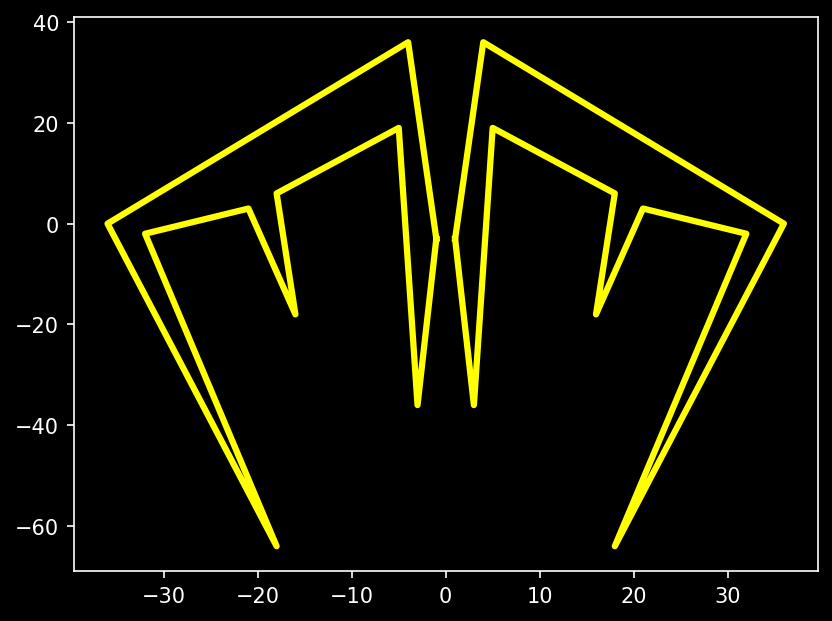
\includegraphics[width=4.22cm]{src/tempest_unused/ENER21.png}%
        \hspace{0.2cm}
        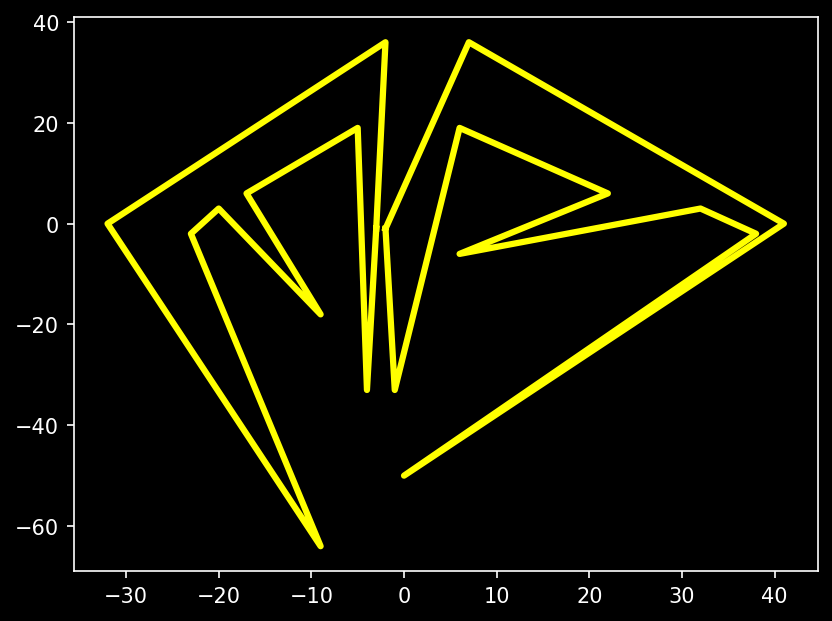
\includegraphics[width=4.22cm]{src/tempest_unused/ENER22.png}%
        \hspace{0.2cm}
        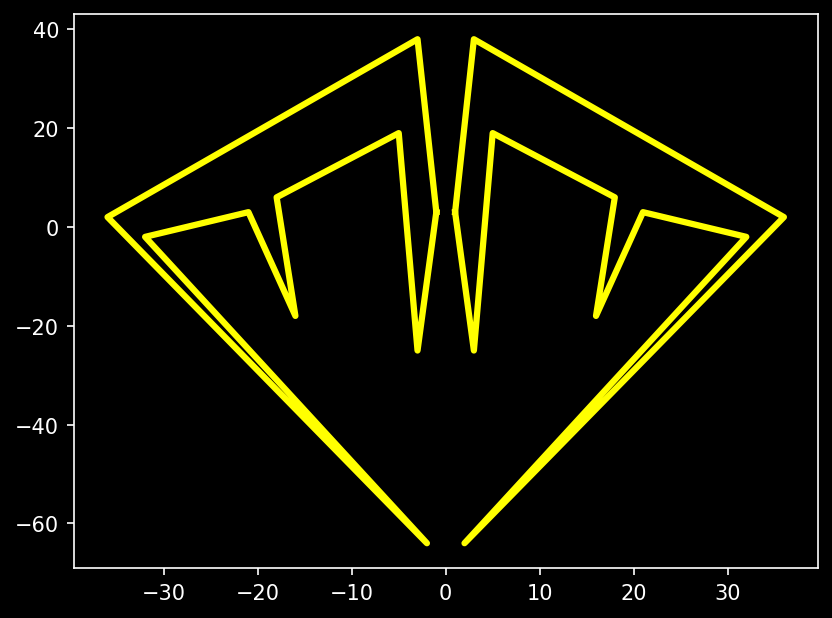
\includegraphics[width=4.22cm]{src/tempest_unused/ENER23.png}%
        \hspace{0.2cm}
        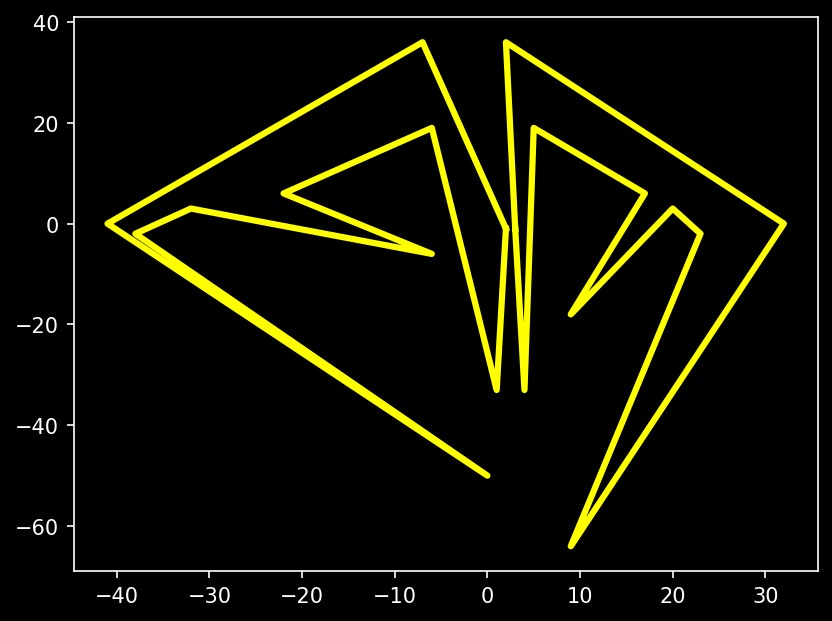
\includegraphics[width=4.22cm]{src/tempest_unused/ENER24.png}%
  \caption*{ENER21 to ENER24 in ALVROM.MAC.}
\end{figure}

\vspace{-0.5cm}
The best of our finds is a clear predecessor to the iconic 'claw' ship. Each is defined
using an array of X/Y co-ordinates that a macro by the name of \icode{CALVEC} encodes into a list
of vector commands. For example, the first image in Figure 2 above is given as follows in
\href{https://github.com/historicalsource/tempest/blob/6c783bee488ed736fc3fdc3a81fdc412c3bec386/ALVROM.MAC#L1483}{\textcolor{blue}{lines 1483-1512} in \icode{ALVROM.MAC}}:
\footnote{https://github.com/historicalsource/tempest/blob/
6c783bee488ed736fc3fdc3a81fdc412c3bec386/
ALVROM.MAC\#L1483}
\begin{lstlisting}
ENER21:
  ICALVE               ; X:0   Y:0     
  CALVEC -1,-3         ; X:-1  Y:-3     
  .BRITE=VARBRT        ; Set brightness to 1
  CALVEC -4,24.        ; X:-4  Y:36
  CALVEC -24.,0        ; X:-36 Y:0
  CALVEC -12.,-40.     ; X:-18 Y:-64
  CALVEC -20.,-2       ; X:-32 Y:-2
  CALVEC -15.,3        ; X:-21 Y:3
  CALVEC -10.,-12.     ; X:-16 Y:-18
  CALVEC -12.,6        ; X:-18 Y:6
  CALVEC -5,13.        ; X:-5  Y:19
  CALVEC -3,-24.       ; X:-3  Y:-36
  CALVEC -1,-3         ; X:-1  Y:-3
  .BRITE=0             ; Set brightness to 0 
  CALVEC 1,-3          ; X:1   Y:-3
  .BRITE=VARBRT        ; Set brightness to 1 
  CALVEC 3,-24.        ; X:3   Y:-36
  CALVEC 5,13.         ; X:5   Y:19
  CALVEC 12.,6         ; X:18  Y:6
  CALVEC 10.,-12.      ; X:16  Y:-18
  CALVEC 15.,3         ; X:21  Y:3
  CALVEC 20.,-2        ; X:32  Y:-2
  CALVEC 12.,-40.      ; X:18  Y:-64
  CALVEC 24.,0         ; X:36  Y:0
  CALVEC 4,24.         ; X:4   Y:36
  CALVEC 1,-3          ; X:1   Y:-3
  .BRITE=0             ; Set brightness to 0 
  CALVEC NXE,0         ; X: 0   Y:0     
  RTSL
\end{lstlisting}

\vspace{0.3cm}
The listing gives X and Y co-ordinates in hex, which we can readily plot as vertices on a graph. During
assembly these values were converted to \href{https://arcarc.xmission.com/Tech/neilw_xy.txt}{\textcolor{blue}{'relative draw'}}\footnote{https://arcarc.xmission.com/Tech/neilw\_xy.txt} vector commands for use by the Atari Analogue Vector Generator (AVG).
These encode \icode{X} and \icode{Y} vectors, along with an intensity value \icode{I} as follows:
\vspace{-0.2cm}
\begin{figure}[H]
  {
    \setlength{\tabcolsep}{3.0pt}
    \setlength\cmidrulewidth{\heavyrulewidth} % Make cmidrule = 
    \begin{adjustbox}{width=8.5cm,center}
      \begin{tabular}{llll}
        \toprule
          &   &   & Vector Command Bits\\
        X & Y & I & \icode{000Y YYYY YYYY YYYY IIIX XXXX XXXX XXXX} \\
        \midrule
        \icode{FF} &\icode{FD} & \icode{00} & \icode{0001 1111 1111 1100 0001 1111 1111 1111} \\
        \addlinespace
        \bottomrule
      \end{tabular}
    \end{adjustbox}
  }
\end{figure}
\vspace{-0.54cm}

The values chosen above are not arbitrary: \icode{X} is -1 (\icode{FF}) and \icode{Y} is -3 (\icode{FD}). Together with an
assumed intensity value of \icode{0} these form the first entry in \icode{ENER21}: \icode{CALVEC -1,-3},
which gets encoded in \href{https://en.wikipedia.org/wiki/Ones%27_complement}{\textcolor{blue}{one's complement}}
\footnote{https://en.wikipedia.org/wiki/Ones\%27\_complement}
for the thirteen bits of each value: \icode{1FFD 1FFF}. 

Let's take that again, step by step. Our command is:
\begin{lstlisting}
  CALVEC -1,-3         ; X:-1  Y:-3     
\end{lstlisting}

This calls the macro \icode{CALVEC} with the values -1 (\icode{FE}) as X and -3 (\icode{FD}) as Y. The end result
we expect from this operation is a vector command that will draw a line from the current point on the screen to the
new co-ordinates. To do this \icode{CALVEC} manipulates the X and Y values we pass relative to the previous position
of X and Y, and offloads the rest of the work to another macro, \icode{VCTR}:

\begin{lstlisting}
        .MACRO CALVEC NEWX,NEWZ
.XN     =NEWX-OLDX      ; Subtract the previous value of X from the current.
.ZN     =NEWZ-OLDZ      ; Subtract the previous value of Y from the current.
VCTR    .XN,.ZN,.BRITE  ; Call the VCTR macro with our new X and Y.
OLDX    =NEWX           ; Store the current X as our previous value.
OLDZ    =NEWZ           ; Store the current Y as our previous value.
        .ENDM
\end{lstlisting}

It is \icode{VCTR} that will transform our humble parameters -1 and 3 into a fully formed 4 byte vector
command. This will be \icode{1FFD1FFF}, let's see how that translation happens:
\begin{lstlisting}
;       VCTR - DRAW VECTOR INSTRUCTION
;       THIS INSTRUCTION DRAWS A VECTOR ON THE DISPLAY AREA
;       RELATIVE TO THE PREVIOUS BEAM POSITION BEFORE THE
;       INSTRUCTION IS EXECUTED.  DX IS THE CHANGE IN BEAM X
;       POSITION; DY IS THE CHANGE IN BEAM Y POSITION; ZZ 
;       SPECIFIES THE BEAM INTENSITY (0 THROUGH 7., 0 IS
;       NO INTENSITY, 7. IS BRIGHTEST INTENSITY).
;
        .SBTTL  VCTR
        .MACRO  VCTR DX,DY,ZZ
        ...1=DX            ; STORE DX AS '1'
        ...2=DY            ; STORE DY AS '2'
        .IF      LT,...1   ; IF NEGATIVE X
        ...1=-DX           ; MAKE IT POSITIVE
        .ENDC              ; END IF
        .IF      LT,...2   ; IF NEGATIVE Y
        ...2=-DY           ; MAKE IT POSITIVE
        .ENDC              ; END IF
        .WORD   DY&^H1FFF,<ZZ*^H2000>+<DX&^H1FFF> ; Turn into a vector command
        .ENDM
\end{lstlisting}
The crux is the penultimate line:
\begin{lstlisting}
        .WORD   DY&^H1FFF,<ZZ*^H2000>+<DX&^H1FFF> ; Turn into a vector command
\end{lstlisting}

The macro assembler computes this into a single line of assembly:
\begin{lstlisting}
        .WORD  1FFD,1FFF 
\end{lstlisting}

Let's see the steps it follows to do this. First we convert each of -1 (\icode{FF}) and
-3 (\icode{FD}) into 'positive' values:
\begin{figure}[H]
  {
    \setlength{\tabcolsep}{3.0pt}
    \setlength\cmidrulewidth{\heavyrulewidth} % Make cmidrule = 
    \begin{adjustbox}{width=7.5cm,center}
      \begin{tabular}{cccc}
        \toprule
        Command  & Left Operand  & Operation  & Result \\
        \midrule
        \icode{...1=-DX} &\icode{FF} & \icode{-} & \icode{00}\\
        \icode{...1=-DY} &\icode{FD} & \icode{-} & \icode{02}\\
        \addlinespace
        \bottomrule
      \end{tabular}
    \end{adjustbox}
  }
\end{figure}

Now we can run the bit operations that will composite everything into a sequence of 4 bytes: 
\begin{figure}[H]
  {
    \setlength{\tabcolsep}{3.0pt}
    \setlength\cmidrulewidth{\heavyrulewidth} % Make cmidrule = 
    \begin{adjustbox}{width=12.5cm,center}
      \begin{tabular}{cccccc}
        \toprule
        Command  & Left Operand  & Operation  & Right Operand & Result & Cumulative Result \\
        \midrule
        \icode{DY\&\string^H1FFF} &\icode{02} & \icode{XOR} & 1FFF & 1FFD & 1FFD0000 \\
        \icode{ZZ*\string^H2000} &\icode{00} & \icode{AND} & 2000 & 0000 & 1FFD0000 \\
        \icode{DX\&\string^H1FFF} &\icode{00} & \icode{XOR} & 1FFF & 0000 & 1FFD1FFF \\
        \addlinespace
        \bottomrule
      \end{tabular}
    \end{adjustbox}
  }
\end{figure}

The successive operations give us our desired result, a vector command that draws a beam line
from the current position to a new position along the vector -1,-3:
\begin{figure}[H]
  {
    \catcode32=\active
    \setlength{\tabcolsep}{3.0pt}
    \setlength\cmidrulewidth{\heavyrulewidth} % Make cmidrule = 
    \begin{adjustbox}{width=8.5cm,center}
      \begin{tabular}{ll}
        \toprule
        Y Value & Intensity/X Value\\
        \midrule
        \icode{   1    F    F    D} & \icode{   1    F    F    F} \\
        \midrule
        \icode{000Y YYYY YYYY YYYY} & \icode{IIIX XXXX XXXX XXXX} \\
        \midrule
        \icode{0001 1111 1111 1100} & \icode{0001 1111 1111 1111} \\
        \addlinespace
        \bottomrule
      \end{tabular}
    \end{adjustbox}
  }
\end{figure}
\vspace{-0.54cm}

There are twelve other finds of interest given below. Unlike the set in Figure 2 above, none of these resemble early
iterations of the player's 'claw'. All our finds appear in an area of the source code described as \icode{ENEMY PICTURES}
and are more likely to be just that: a set of alien enemies for a very early iteration of Tempest that according to
programmer David Theurer was a 
\href{https://arcadeblogger.com/2018/01/19/atari-tempest-dave-theurers-masterpiece/}{\textcolor{blue}{‘First Person Space Invaders’}}.
\footnote{https://arcadeblogger.com/2018/01/19/atari-tempest-dave-theurers-masterpiece/}

\begin{figure}[H]
  \centering
        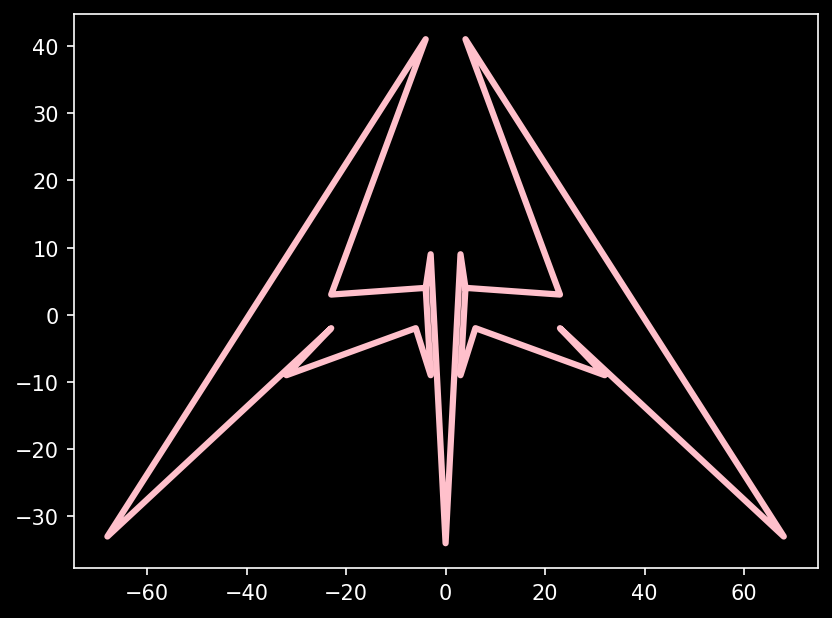
\includegraphics[width=4.22cm]{src/tempest_unused/ENER11.png}%
        \hspace{0.2cm}
        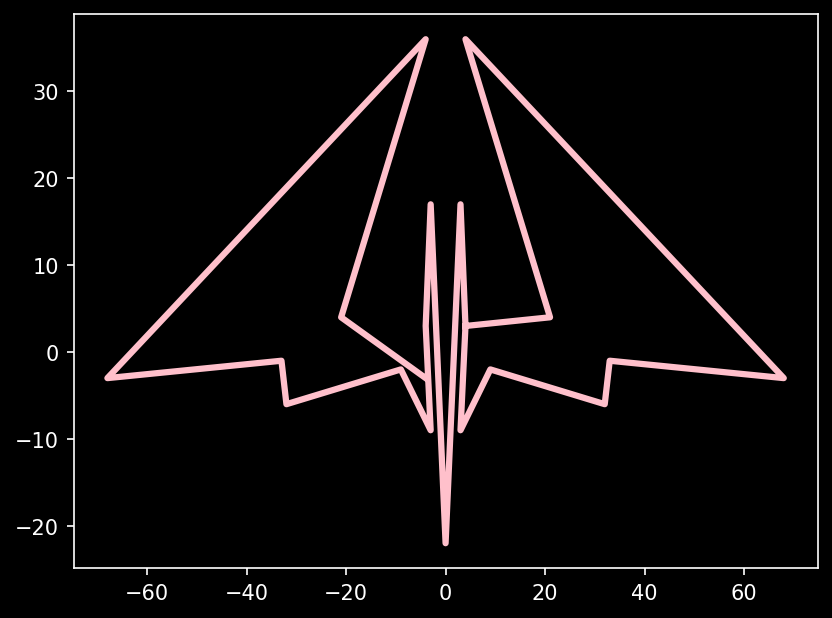
\includegraphics[width=4.22cm]{src/tempest_unused/ENER12.png}%
        \hspace{0.2cm}
        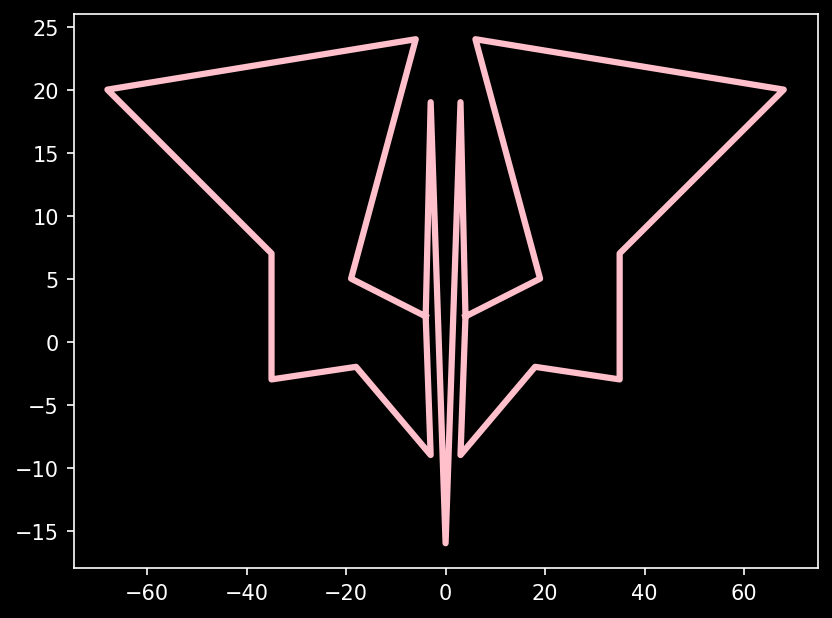
\includegraphics[width=4.22cm]{src/tempest_unused/ENER13.png}%
        \hspace{0.2cm}
        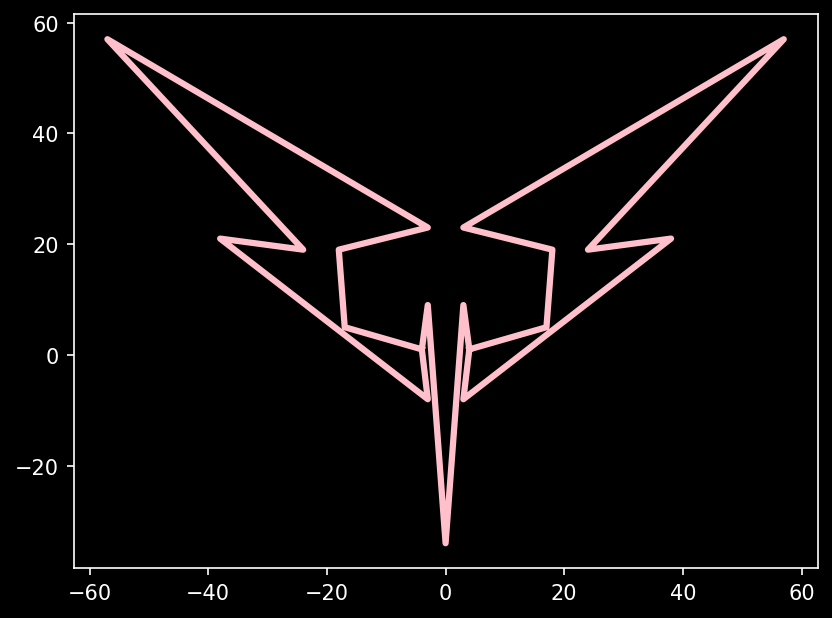
\includegraphics[width=4.22cm]{src/tempest_unused/ENER14.png}%
  \caption*{ENER11 to ENER14 in ALVROM.MAC.}
\end{figure}
\begin{figure}[H]
  \centering
        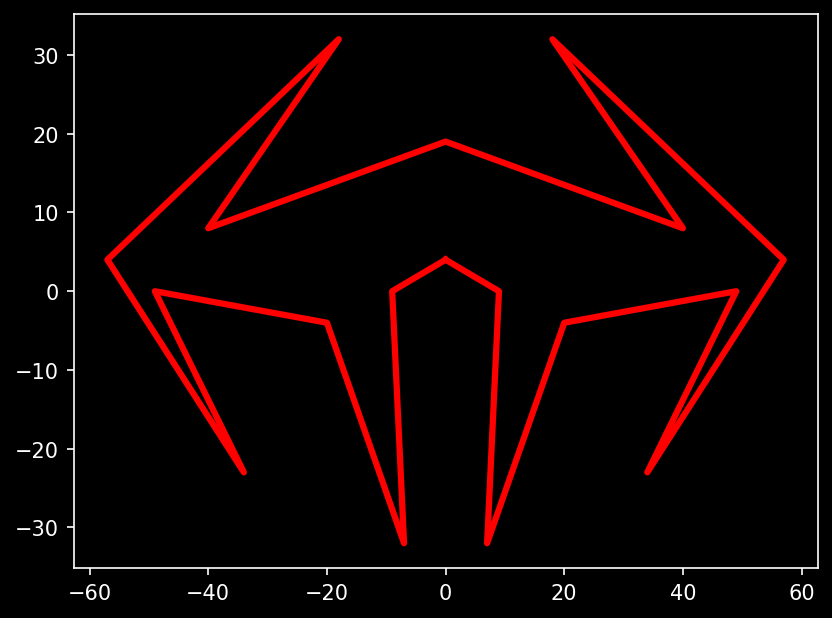
\includegraphics[width=4.22cm]{src/tempest_unused/ENER41.png}%
        \hspace{0.2cm}
        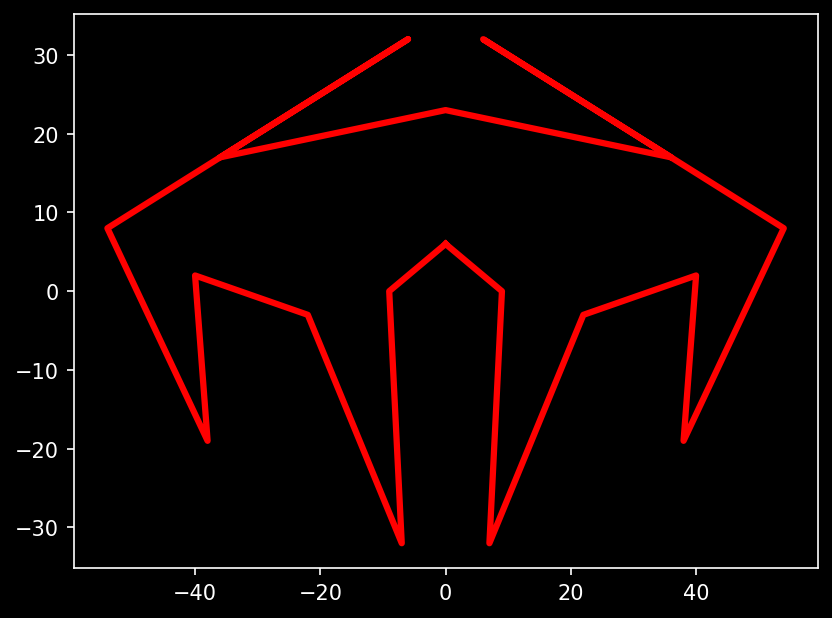
\includegraphics[width=4.22cm]{src/tempest_unused/ENER42.png}%
        \hspace{0.2cm}
        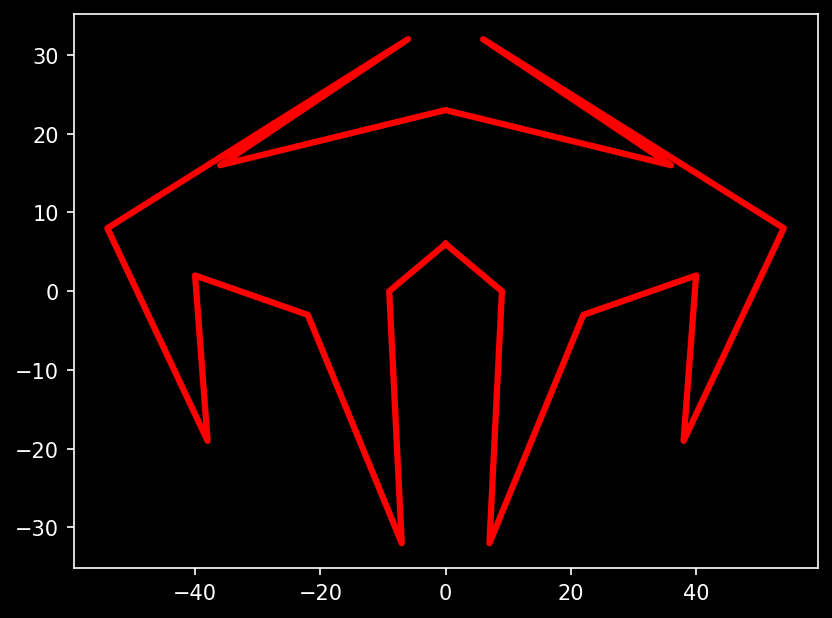
\includegraphics[width=4.22cm]{src/tempest_unused/ENER43.png}%
        \hspace{0.2cm}
        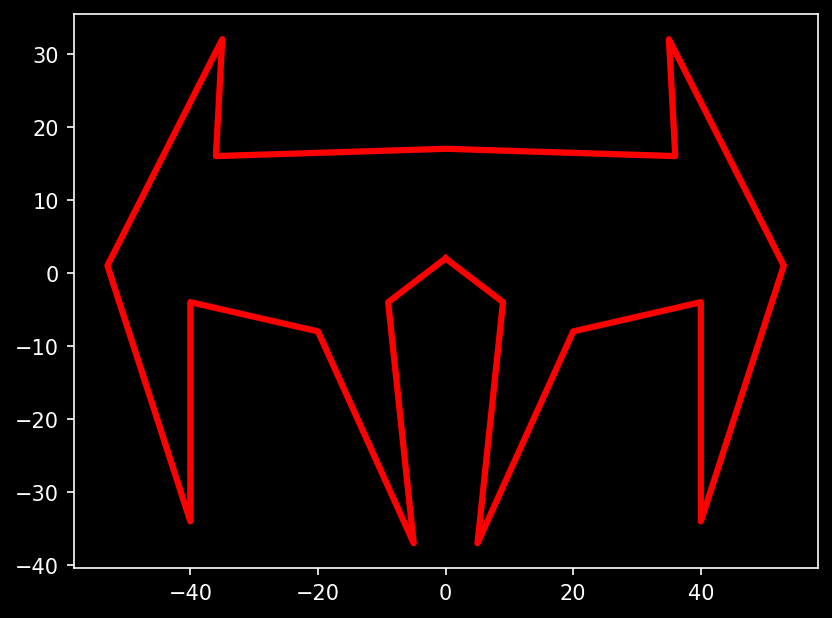
\includegraphics[width=4.22cm]{src/tempest_unused/ENER44.png}%
  \caption*{ENER41 to ENER44 in ALVROM.MAC.}
\end{figure}
\begin{figure}[H]
  \centering
        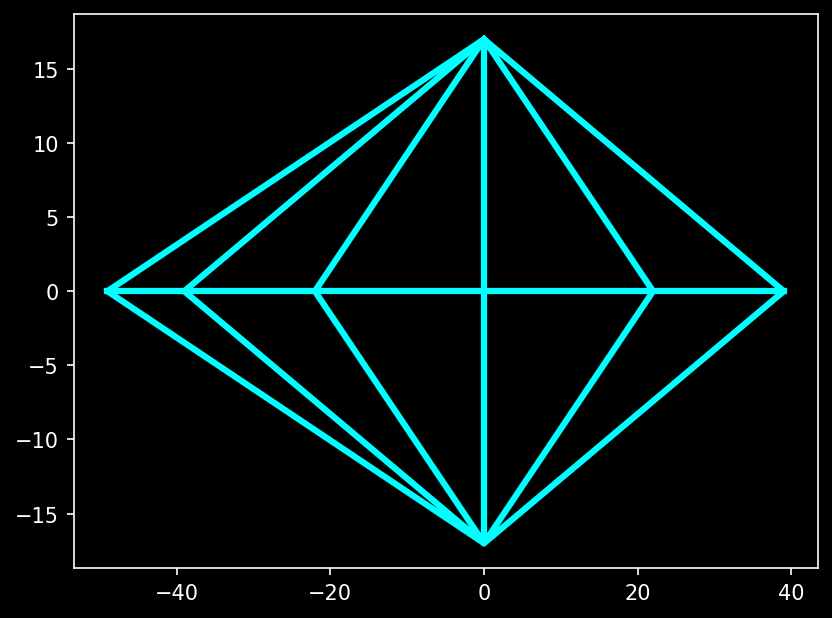
\includegraphics[width=4.22cm]{src/tempest_unused/SAU.png}%
        \hspace{0.2cm}
        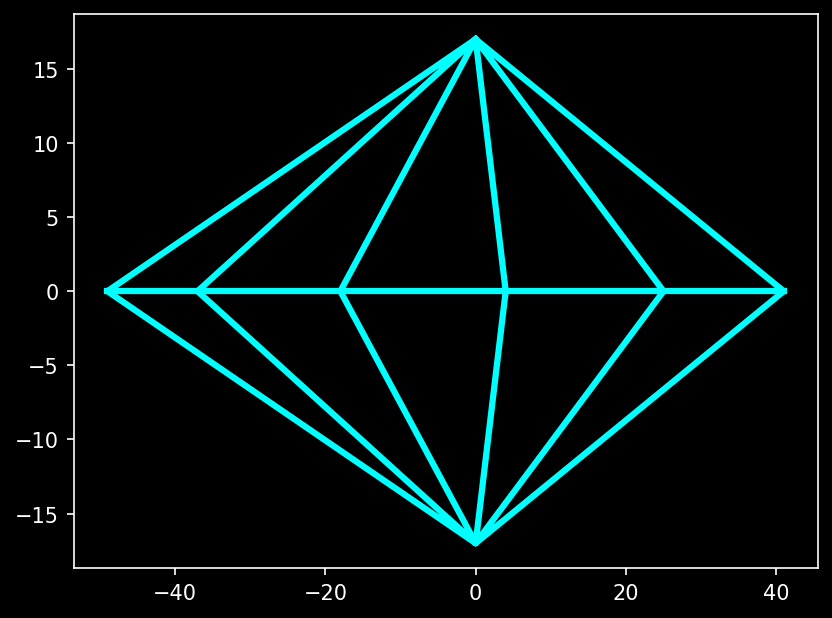
\includegraphics[width=4.22cm]{src/tempest_unused/SA2.png}%
        \hspace{0.2cm}
        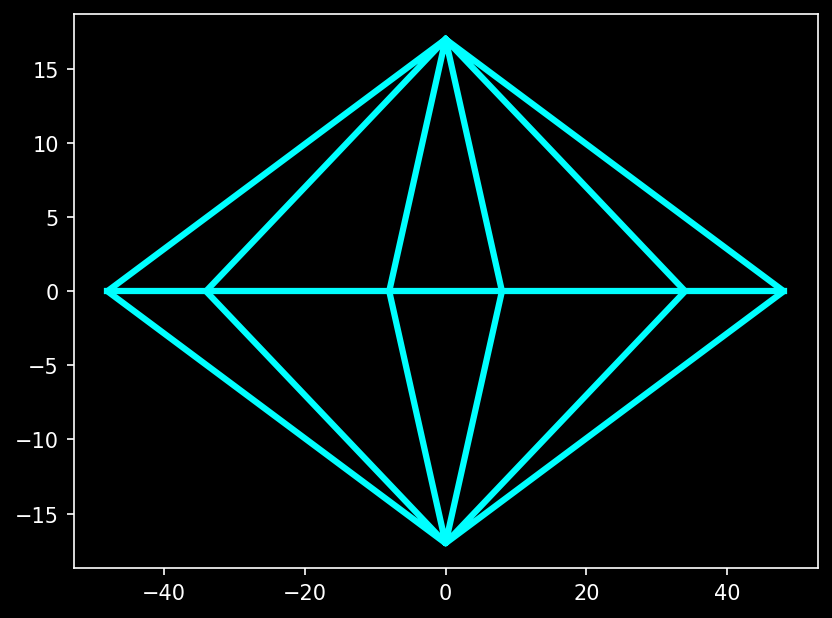
\includegraphics[width=4.22cm]{src/tempest_unused/SA3.png}%
        \hspace{0.2cm}
        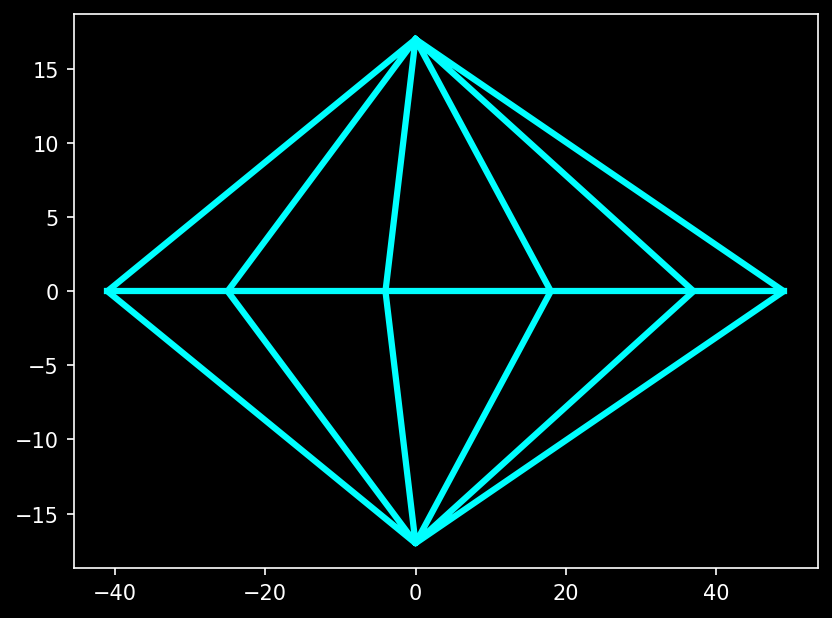
\includegraphics[width=4.22cm]{src/tempest_unused/SA4.png}%
  \caption*{SAU to SA4 in ALVROM.MAC.}
\end{figure}

